\section{Các bài kiểm tra}
Thông qua cuộc khảo sát, nhóm còn nhận thấy một số kết quả bất ngờ khác về kết quả khảo sát của các bài kiểm tra

\begin{figure}[H]
    \centering
    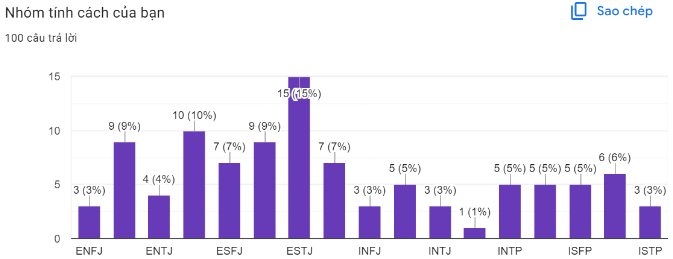
\includegraphics[width=0.8\linewidth]{images/survey2.png}    \vspace{0.6cm}
    \caption{Khảo sát về bài kiểm tra MBTI}
\end{figure}

Nhóm tính cách phổ biến nhất trong những cá nhân thực hiện khảo sát là ESTJ, với một tỉ lệ là 15\% .Và đặc biệt các nhóm tính cách có chữ T - Thinking, vốn là các nhóm tính cách có thế mạnh thiên về suy nghĩ logic trong cặp đối lập Thinking-Feeling logic hay cảm xúc, thì T là tính cách chiếm số lượng vượt trội hơn hẳn. Điều này cũng hoàn toàn trùng khớp với kết quả nghiên cứu về nhóm tính cách của kĩ sư tại Trường đại học Bách Khoa có đề xuất ở lần trước về nhóm tính cách S-T chiếm tỉ trọng lớn nhất.

Ngoài ra, tỉ lệ nhóm ngành kĩ thuật vẫn chiếm tỉ lệ lớn nhất trong các cụm ngành nghề được phân theo phương pháp Career Clustering

\begin{figure}[H]
    \centering
    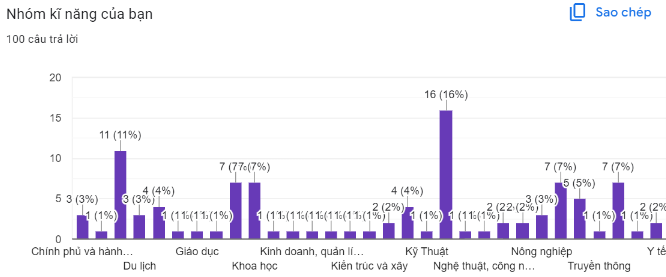
\includegraphics[width=0.8\linewidth]{images/survey3.png}    \vspace{0.6cm}
    \caption{Khảo sát về bài kiểm tra Career Clustering}
\end{figure}

Điều này có thể lí giải dễ dàng vì Bách Khoa Thành Phố Hồ Chí Minh là môi trường kỹ thuật thuộc top đầu cả nước. Do đó những sinh viên cũng sẽ có xu hướng về các ngành kĩ thuật, công nghệ, khoa học và ít xuất hiện nhóm ngành kinh tế, đặc biệt là những nhóm ngành đặc thù như tài chính thì lại càng ít xuất hiện.

Hai phân tích thú vị trên cũng phản ánh rằng, khảo sát này chỉ là con số ban đầu, chưa thể có một kết luận sâu rộng hơn khi áp dụng rộng rãi đối với các nhóm ngành đặc thù về kinh tế, tài chính cần có những khảo sát toàn diện hơn để có thể đánh giá được tính chính xác của hệ thống.
